% vggmm_vs_bgm.tex -- VGGMM(구조 이동 포함) vs BGM 비교 보고
% 컴파일: XeLaTeX (Overleaf: Menu -> Compiler -> XeLaTeX). 그림·표 파일은 같은 폴더에 둔다.
\documentclass[11pt]{article}
\usepackage{kotex}
\usepackage[a4paper,margin=22mm]{geometry}
\usepackage{amsmath,amssymb}
\usepackage{booktabs,graphicx}
\renewcommand{\arraystretch}{1.15}
\setlength{\parskip}{4pt}

\title{GGD 혼합(VGGMM)과 BGM의 밀도 추정 비교\\[2pt]\large 다양한 분포·표본 수·실데이터와 $K_{\max}$ 분석}
\author{}
\date{}

\begin{document}
\maketitle

\section{요약}

CTGAN 전처리의 BGM(Gaussian 성분, rdt 설정)과, 성분을 일반화 정규분포(GGD)로 바꾸고 ELBO로 검증하는 구조 이동(병합·삭제·재정렬)을 더한 VGGMM을 같은 조건에서 비교했다. $K_{\max}=10$은 rdt 기본값이다.

\begin{itemize}
  \item \textbf{GGD로 표현되는 분포에서 정확도 차이가 크다.}
    \begin{itemize}
      \item 꼬리가 두꺼운 혼합, 윗부분이 평평한 혼합, 섞인 5성분 혼합에서 VGGMM은 27번 비교에서 모두 이겼다.
      \item 참 분포와의 KL은 BGM보다 중앙값 기준 15--32배 작다.
      \item GGD 밖의 분포인 균등분포 블록에서도 9번 모두 이겼다(5.7배).
    \end{itemize}
  \item \textbf{성분 수가 $K_{\max}$에 끌려가지 않는다.}
    \begin{itemize}
      \item 참 성분이 3개인 정규 혼합에서 $K_{\max}=5\to50$으로 늘리면, BGM의 유효 성분은 $5\to18$로 늘어난다. VGGMM은 모든 $K_{\max}$에서 3이다.
      \item adult age에서는 BGM이 $5\to42$, VGGMM이 4--6이다.
      \item BGM이 더 쓴 성분은 평가 로그우도를 높이지 못했다.
    \end{itemize}
  \item \textbf{실데이터(표본 1.6--1.9만)에서 10개 열 중 9개 열이 3개 시드 모두 우세하다.} 나머지 1개 열도 차이가 0.001 이하다.
  \item \textbf{약점.}
    \begin{itemize}
      \item 표본이 적을 때($n=1000$의 정규·겹친 혼합, breast cancer $n=284$) BGM보다 약간 나쁘다.
      \item 비대칭(로그정규)과 다항 꼬리(Student-$t$) 분포에서는 BGM과 비슷하거나 조금 나쁘다.
      \item 학습 시간은 BGM보다 길다. 중앙값 기준으로 인공 데이터에서 약 7배, 실데이터(1.6--1.9만 행)에서 약 16배이고, $K_{\max}$에 대해 거의 제곱으로 늘어난다.
    \end{itemize}
\end{itemize}

\section{비교 설정}

\begin{center}\small
\begin{tabular}{p{3.0cm}p{12.0cm}}
\toprule
BGM & sklearn \texttt{BayesianGaussianMixture}, DP 사전 $\gamma=0.001$, $K_{\max}=10$ (rdt \texttt{ClusterBasedNormalizer}와 같은 설정) \\
VGGMM & GGD 성분, $q(\tau)$ Gamma 켤레, $\mu,\beta$ 점추정, ELBO로 검증하는 병합·삭제·재정렬 이동, $K_{\max}=10$ \\
인공 분포 & 8종: GGD 혼합 5종(정규, 꼬리가 두꺼움, 윗부분이 평평함, 섞인 5성분, 많이 겹침)과 GGD 밖의 분포 3종($^{*}$: Student-$t$ 혼합, 로그정규, 균등분포 블록) \\
표본 수와 시드 & $n\in\{1000,5000,20000\}$, 시드 3개. 평가 데이터 2만 개는 따로 생성 \\
실데이터 & adult 6열($n=32{,}561$), br2000 연속 4열($n=38{,}000$), breast cancer 4열($n=569$). 50/50 분할, 시드 3개. 정수 열은 두 방법에 같은 디퀀타이즈를 적용 \\
지표 & 인공 분포: KL$=\overline{\log p_{\text{true}}}-\overline{\log p_{\text{model}}}$(작을수록 좋음), IAE. 실데이터: 평가 표본당 로그우도(클수록 좋음). 공통: 유효 성분 수($\hat\pi_k>0.005$), 학습 시간 \\
\bottomrule
\end{tabular}
\end{center}

\section{인공 분포}

\begin{figure}[h!]
\centering
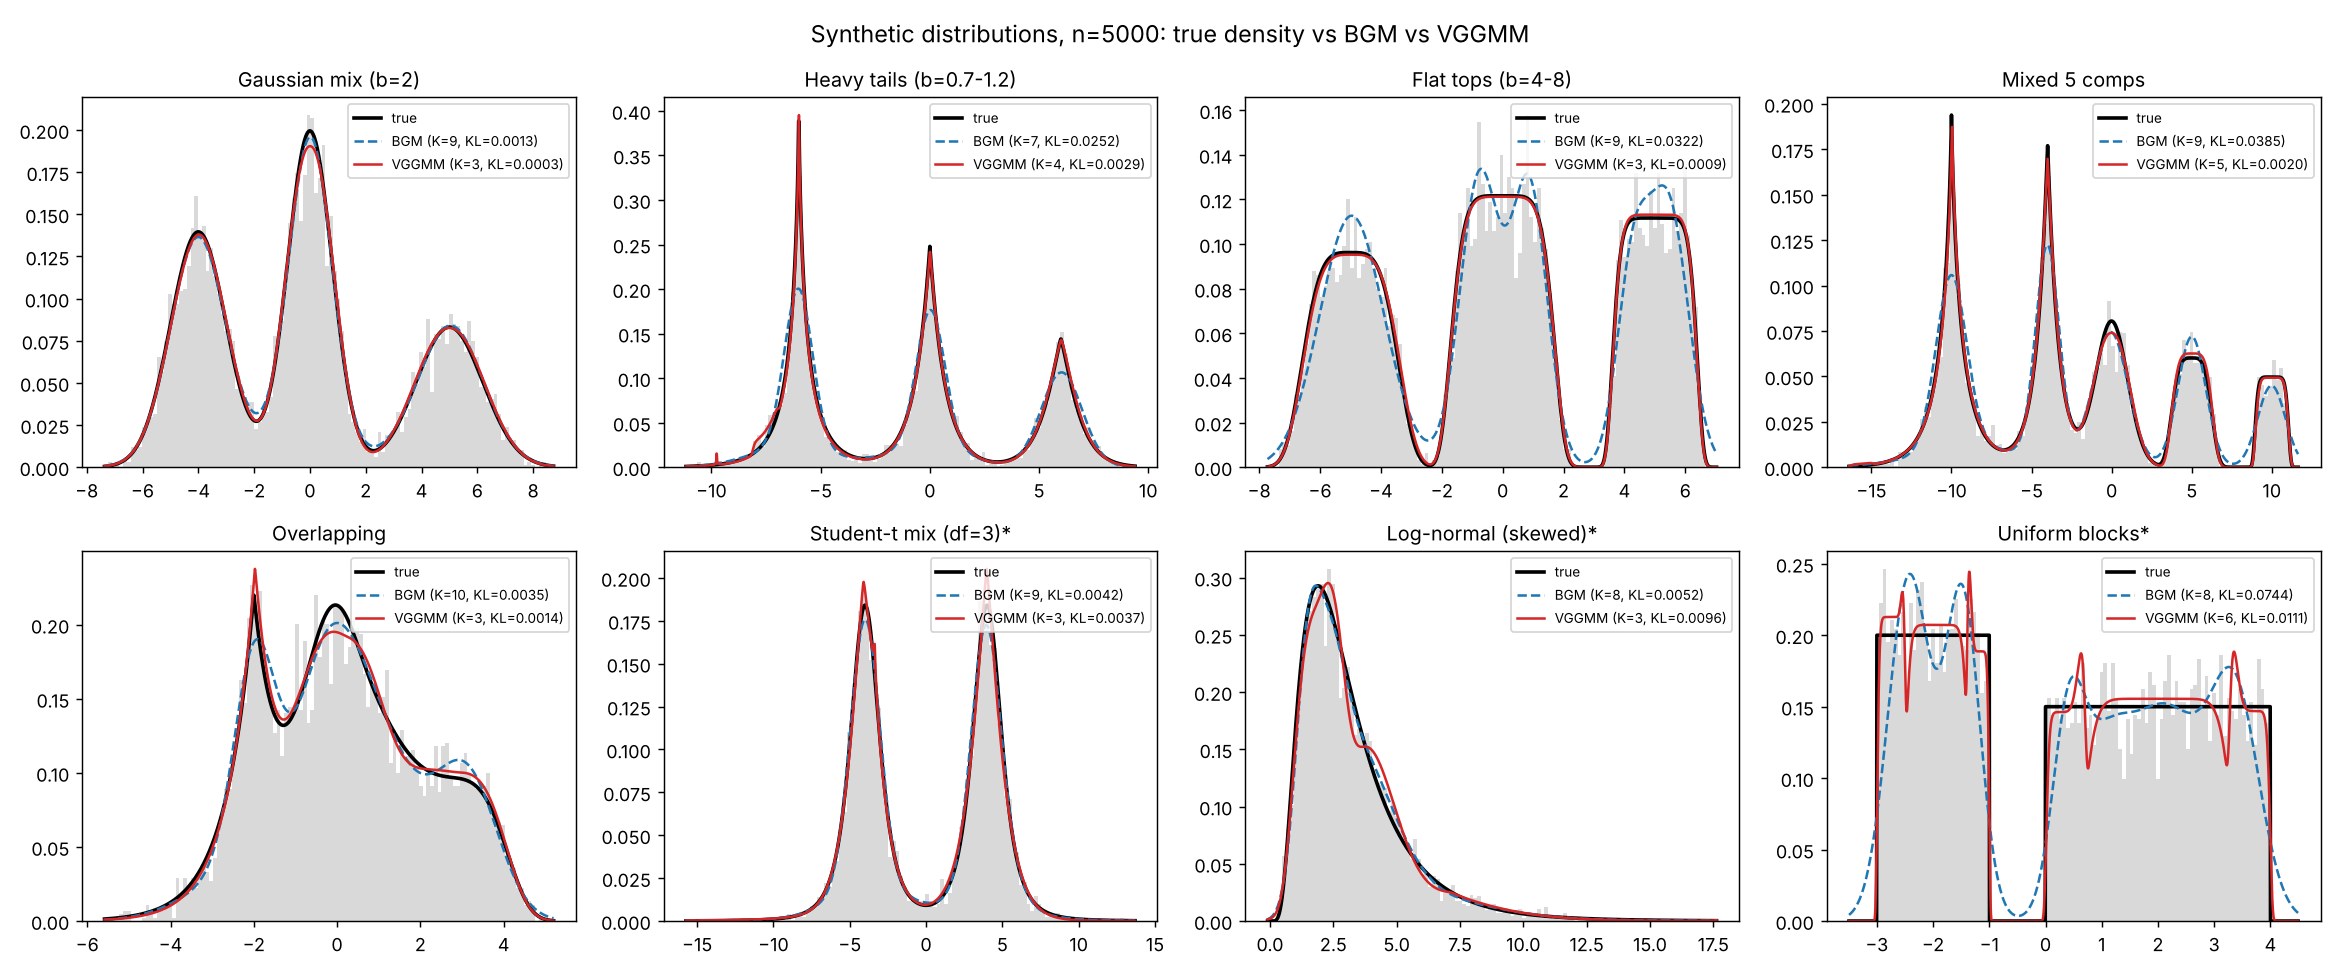
\includegraphics[width=\textwidth]{fig_synth_overlay.png}
\caption{$n=5000$, 시드 0. 회색은 표본 히스토그램, 검정은 참 밀도, 파란 점선은 BGM, 빨간 실선은 VGGMM이다. 범례의 $K$는 유효 성분 수다.}
\end{figure}

그림에서 볼 수 있듯이, BGM은 뾰족한 봉우리를 낮게 뭉개고, 평평한 윗부분을 Gaussian 여러 개로 물결처럼 흉내 내며, 상자 경계 밖으로 퍼진다. VGGMM은 형상 $\beta$로 이런 모양을 한 성분이 직접 표현한다.

\begin{figure}[h!]
\centering
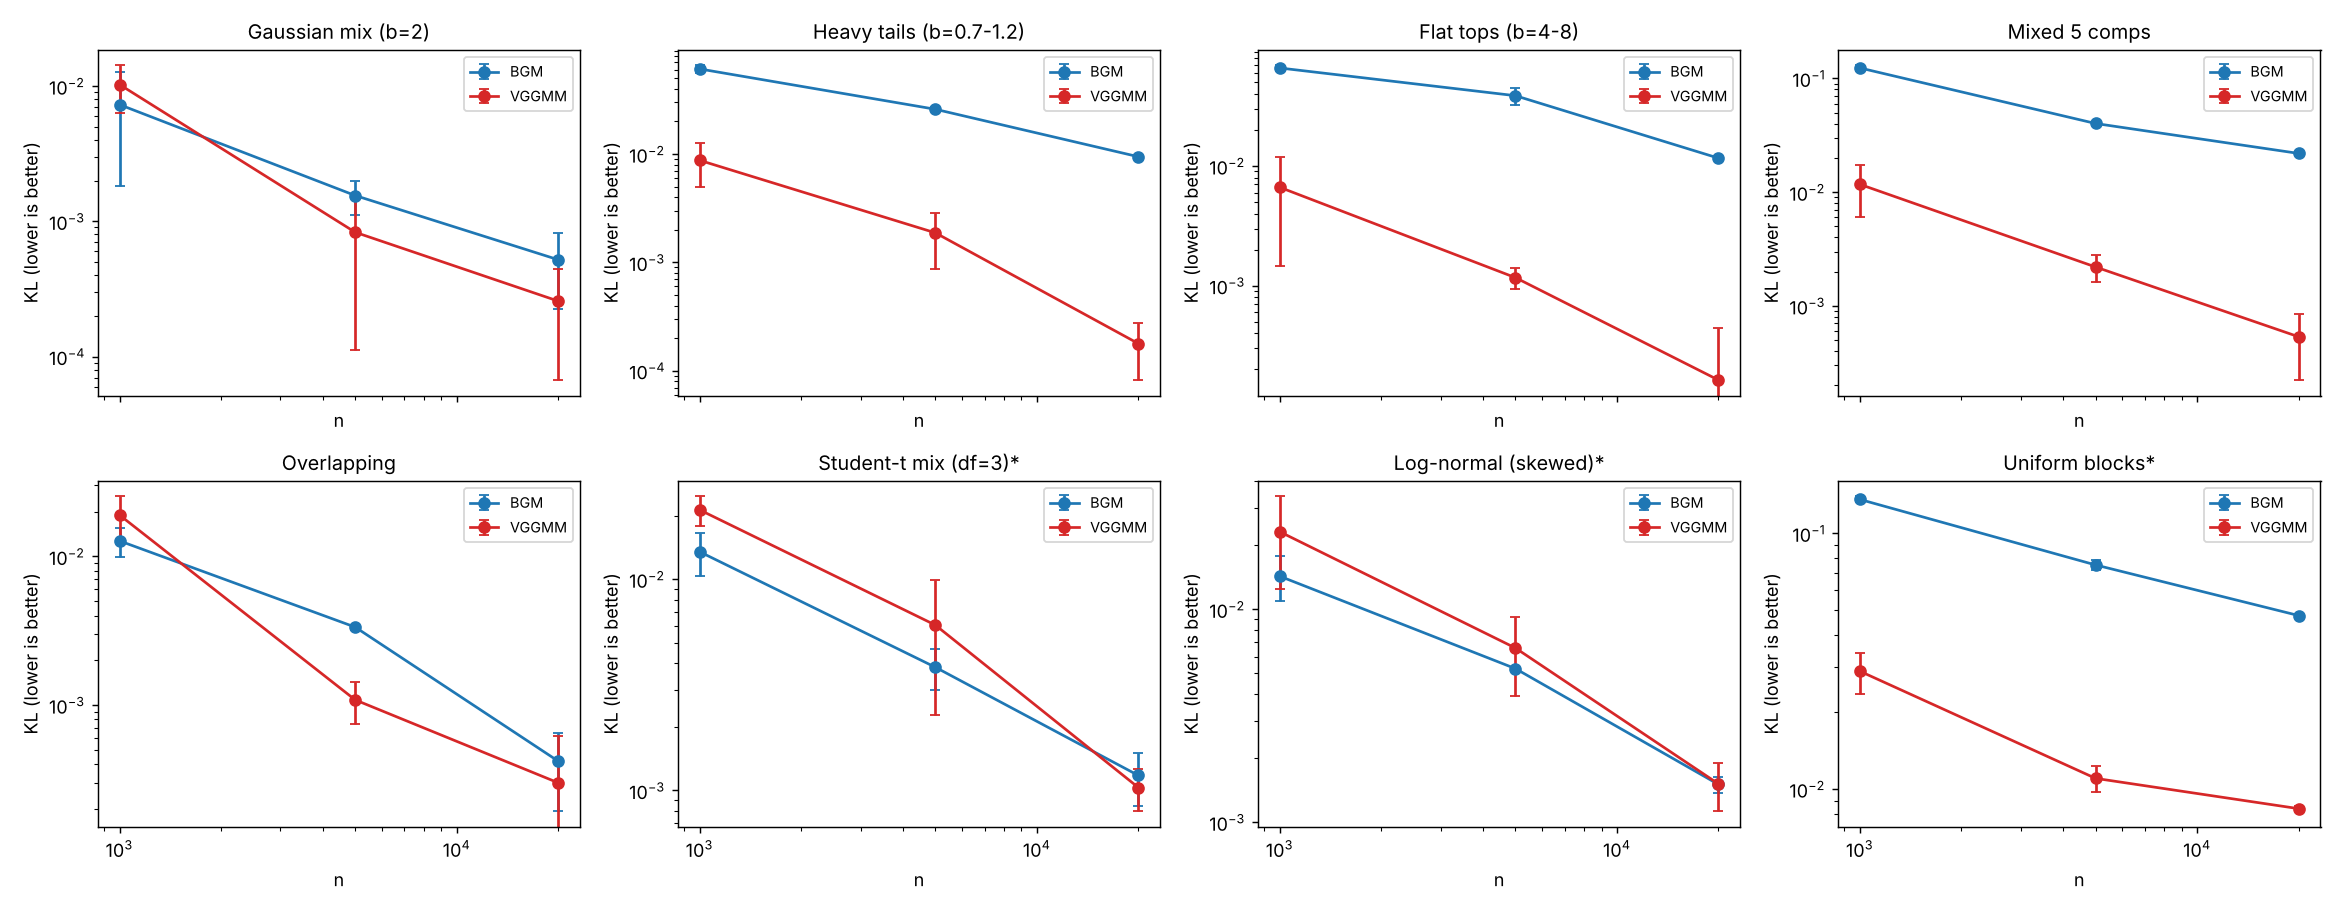
\includegraphics[width=\textwidth]{fig_synth_kl.png}
\caption{표본 수에 따른 KL(로그 눈금, 시드 3개의 평균$\pm$표준편차).}
\end{figure}

\begin{table}[h!]
\centering\small
\begin{tabular}{lrrrrrrr}
\toprule
분포 & $n$ & KL BGM & KL VGGMM & 비율 & 승 & $K$ BGM & $K$ VGGMM \\
\midrule
Gaussian mix (b=2) & 1000 & 0.0073 & 0.0103 & 0.6 & 0/3 & 3.3 & 3.0 \\
 & 5000 & 0.0016 & 0.0008 & 2.7 & 3/3 & 8.0 & 3.0 \\
 & 20000 & 0.0005 & 0.0003 & 1.9 & 3/3 & 10.0 & 3.0 \\
\addlinespace
Heavy tails (b=0.7-1.2) & 1000 & 0.0610 & 0.0088 & 6.3 & 3/3 & 4.3 & 3.0 \\
 & 5000 & 0.0259 & 0.0019 & 14.9 & 3/3 & 7.3 & 3.3 \\
 & 20000 & 0.0095 & 0.0002 & 63.6 & 3/3 & 10.0 & 3.0 \\
\addlinespace
Flat tops (b=4-8) & 1000 & 0.0659 & 0.0066 & 16.2 & 3/3 & 4.0 & 3.0 \\
 & 5000 & 0.0387 & 0.0012 & 33.6 & 3/3 & 9.0 & 3.0 \\
 & 20000 & 0.0116 & 0.0002 & $>$100 & 3/3 & 10.0 & 3.0 \\
\addlinespace
Mixed 5 comps & 1000 & 0.1236 & 0.0117 & 14.0 & 3/3 & 6.0 & 5.0 \\
 & 5000 & 0.0402 & 0.0022 & 19.1 & 3/3 & 9.0 & 5.0 \\
 & 20000 & 0.0219 & 0.0005 & 51.1 & 3/3 & 9.7 & 5.0 \\
\addlinespace
Overlapping & 1000 & 0.0127 & 0.0190 & 0.7 & 0/3 & 5.7 & 2.0 \\
 & 5000 & 0.0033 & 0.0011 & 3.1 & 3/3 & 10.0 & 3.0 \\
 & 20000 & 0.0004 & 0.0003 & 2.0 & 3/3 & 10.0 & 3.0 \\
\addlinespace
Student-t mix (df=3)$^{*}$ & 1000 & 0.0135 & 0.0213 & 0.8 & 0/3 & 4.0 & 2.0 \\
 & 5000 & 0.0038 & 0.0061 & 1.1 & 2/3 & 9.0 & 3.0 \\
 & 20000 & 0.0012 & 0.0010 & 0.9 & 1/3 & 9.7 & 3.7 \\
\addlinespace
Log-normal (skewed)$^{*}$ & 1000 & 0.0143 & 0.0231 & 0.6 & 0/3 & 6.0 & 3.0 \\
 & 5000 & 0.0053 & 0.0066 & 0.9 & 1/3 & 8.3 & 3.7 \\
 & 20000 & 0.0015 & 0.0015 & 0.9 & 1/3 & 9.0 & 5.3 \\
\addlinespace
Uniform blocks$^{*}$ & 1000 & 0.1357 & 0.0289 & 4.8 & 3/3 & 4.3 & 3.7 \\
 & 5000 & 0.0752 & 0.0110 & 6.7 & 3/3 & 8.7 & 6.3 \\
 & 20000 & 0.0477 & 0.0084 & 5.7 & 3/3 & 10.0 & 7.7 \\
\addlinespace
\bottomrule
\end{tabular}
\caption{인공 분포 결과. ``비율''은 BGM KL / VGGMM KL의 중앙값으로, 1보다 크면 VGGMM이 참 분포에 더 가깝다. VGGMM의 KL이 거의 0이면 비율이 부풀려지므로 100을 넘는 값은 $>$100으로 표시했다. ``승''은 시드 3개 중 VGGMM의 KL이 더 작은 횟수다.}
\end{table}

\paragraph{정리.}
\begin{itemize}
  \item 72번 비교 중 VGGMM이 53번 이겼다(74\%).
  \item GGD 혼합 5종에서는 45번 중 39번, GGD 밖의 분포 3종에서는 27번 중 14번 이겼다.
  \item 표본 수별로는 $n=1000$에서 24번 중 12번, $n=5000$에서 21번, $n=20000$에서 20번 이겼다.
  \item VGGMM의 유효 성분 수는 참 성분 수(3 또는 5)에 가깝다. BGM은 평균 7--9개를 썼다.
\end{itemize}

\clearpage
\section{실데이터}

\begin{figure}[h!]
\centering
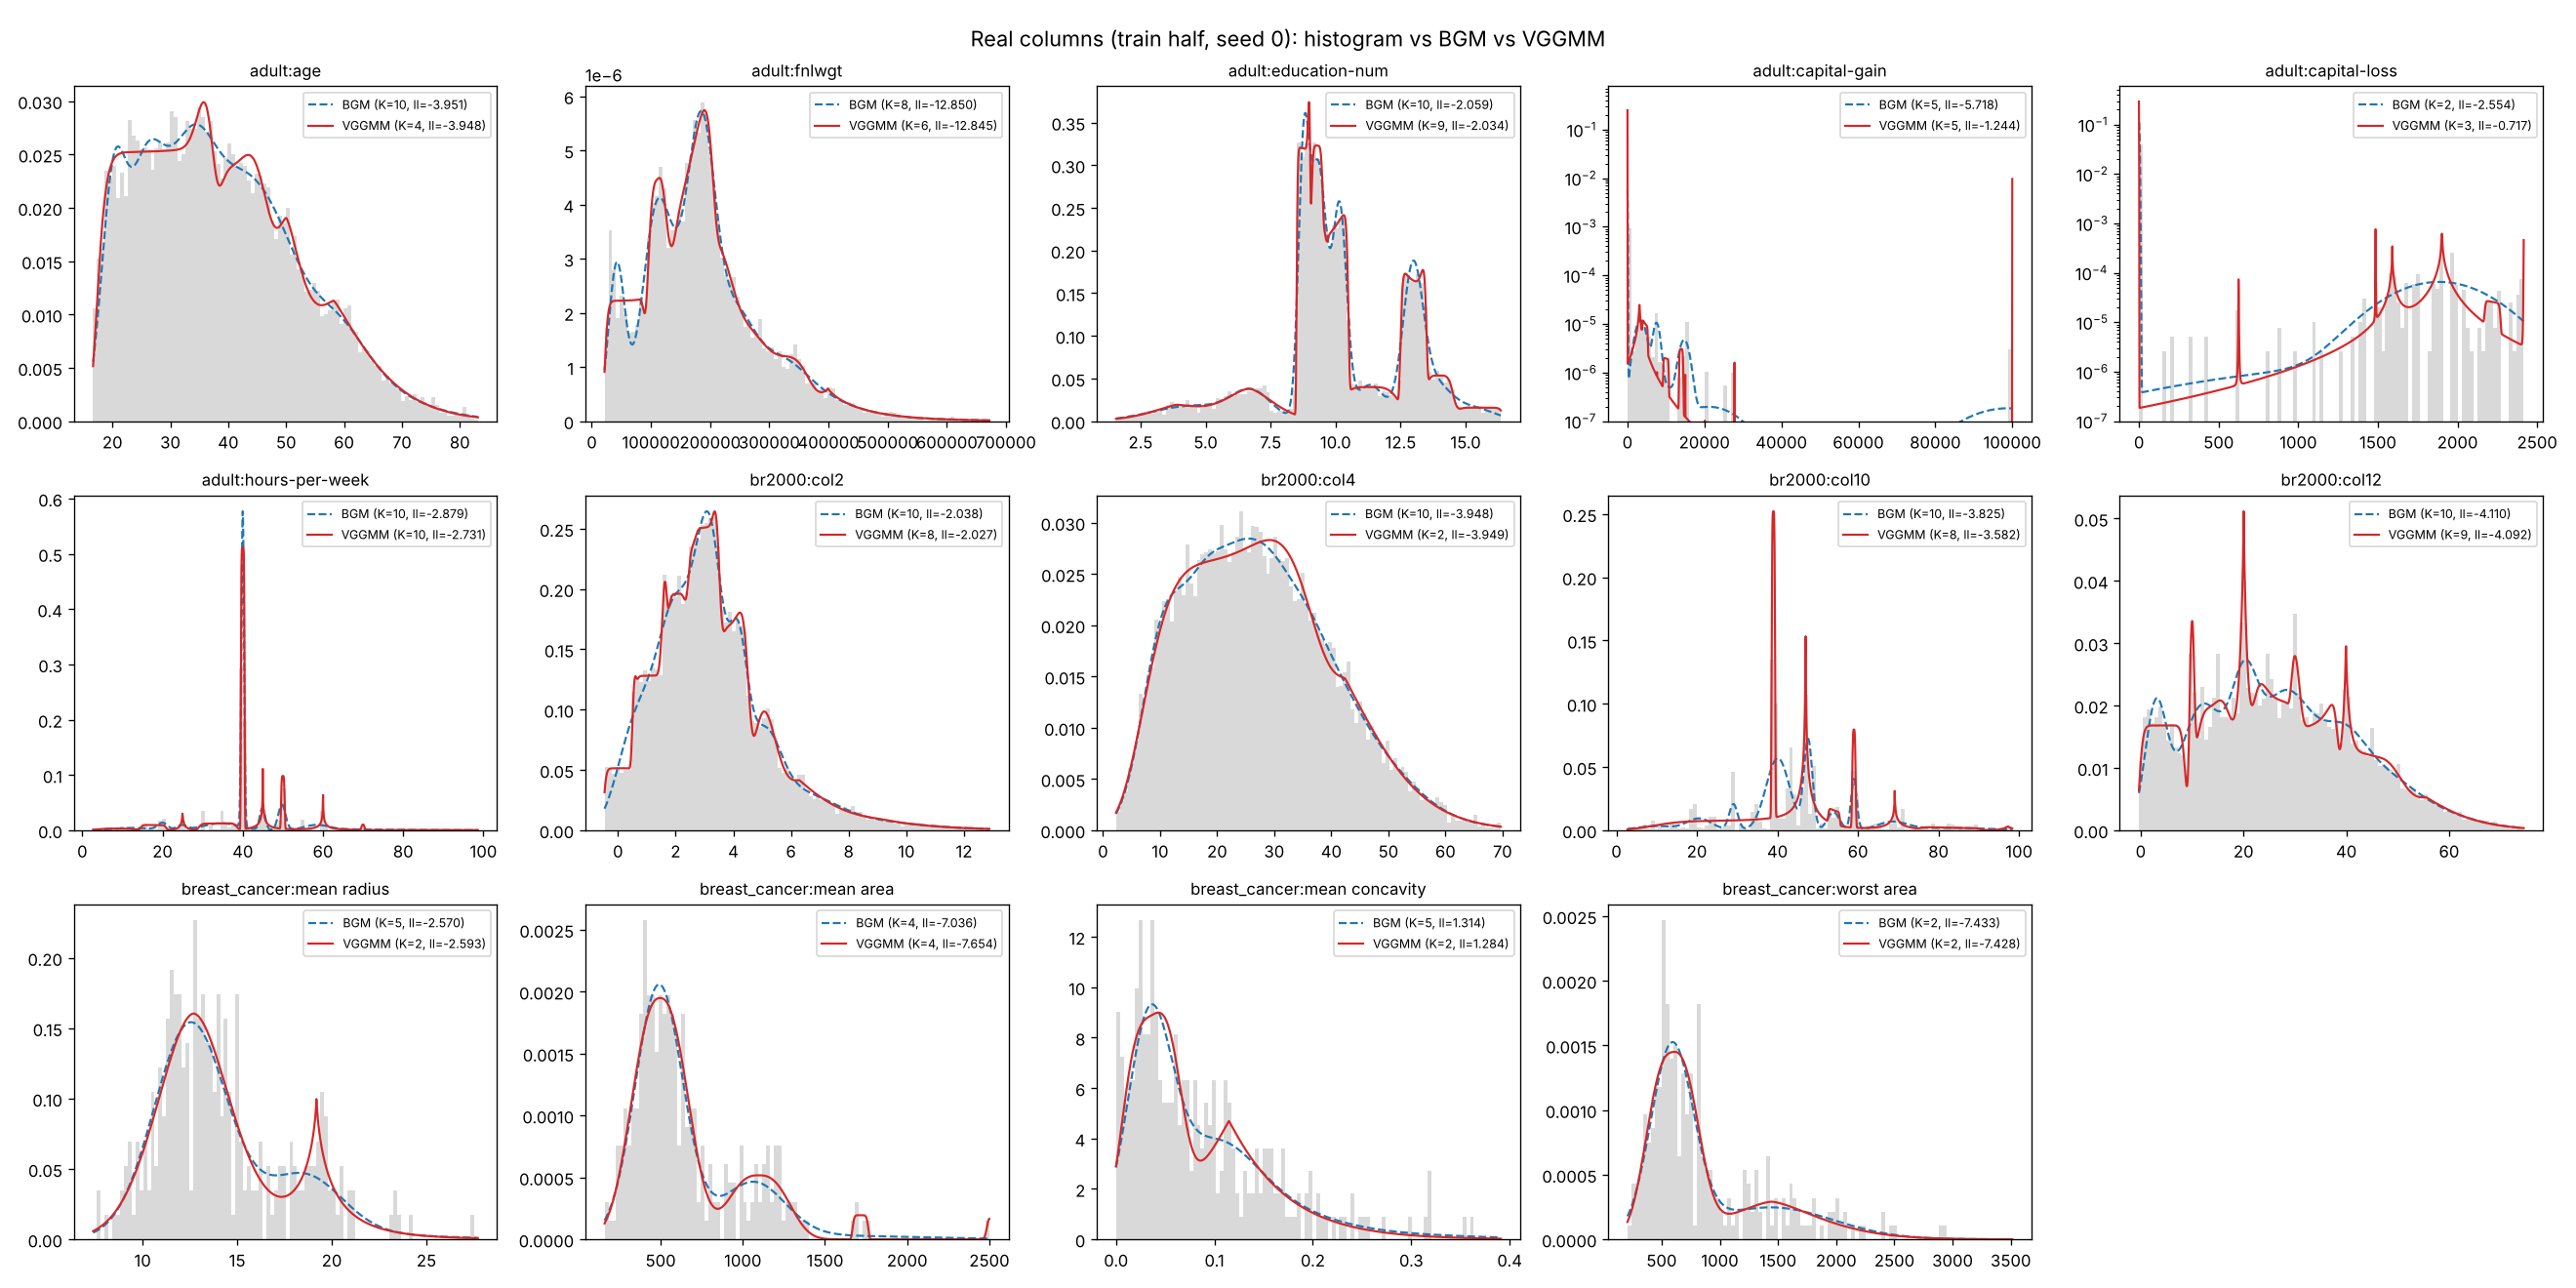
\includegraphics[width=\textwidth]{fig_real_overlay.png}
\caption{학습 절반(시드 0)의 히스토그램과 두 모형의 밀도. capital-gain과 capital-loss는 0이 90\% 이상이라 $y$축을 로그 눈금으로 그렸다.}
\end{figure}

\begin{table}[h!]
\centering
\resizebox{\textwidth}{!}{\begin{tabular}{lrrrrrrrr}
\toprule
열 & $n_{\mathrm{train}}$ & ll BGM & ll VGGMM & 차이 & 승 & $K$ BGM & $K$ VGGMM & 시간(s) BGM/VGGMM \\
\midrule
adult:age & 16280 & -3.951 & -3.947 & +0.004 & 3/3 & 10.0 & 4.0 & 0.8/15.8 \\
adult:fnlwgt & 16280 & -12.847 & -12.841 & +0.006 & 3/3 & 8.7 & 6.0 & 0.8/16.2 \\
adult:education-num & 16280 & -2.069 & -2.042 & +0.028 & 3/3 & 10.0 & 9.0 & 0.8/11.4 \\
adult:capital-gain & 16280 & -5.737 & -1.261 & +4.477 & 3/3 & 5.0 & 5.7 & 0.8/3.6 \\
adult:capital-loss & 16280 & -2.545 & -0.708 & +1.838 & 3/3 & 2.3 & 4.0 & 0.7/4.4 \\
adult:hours-per-week & 16280 & -2.890 & -2.751 & +0.139 & 3/3 & 10.0 & 9.7 & 0.9/10.8 \\
br2000:col2 & 19000 & -2.042 & -2.030 & +0.013 & 3/3 & 9.7 & 8.3 & 0.9/17.2 \\
br2000:col4 & 19000 & -3.948 & -3.949 & -0.001 & 0/3 & 10.0 & 2.0 & 0.9/14.4 \\
br2000:col10 & 19000 & -3.688 & -3.523 & +0.165 & 3/3 & 10.0 & 9.3 & 0.9/13.5 \\
br2000:col12 & 19000 & -4.111 & -4.095 & +0.017 & 3/3 & 10.0 & 7.7 & 0.9/17.7 \\
breast\_cancer:mean radius & 284 & -2.555 & -2.563 & -0.008 & 1/3 & 3.7 & 2.0 & 0.1/0.7 \\
breast\_cancer:mean area & 284 & -7.012 & -7.217 & -0.205 & 1/3 & 3.7 & 3.0 & 0.0/0.7 \\
breast\_cancer:mean concavity & 284 & 1.359 & 1.350 & -0.010 & 1/3 & 4.0 & 2.7 & 0.0/0.9 \\
breast\_cancer:worst area & 284 & -7.401 & -7.410 & -0.009 & 1/3 & 3.0 & 2.0 & 0.1/0.6 \\
\bottomrule
\end{tabular}}
\caption{실데이터 결과(시드 3개 평균). ``차이''는 VGGMM $-$ BGM의 평가 로그우도이고, 양수이면 VGGMM이 낫다.}
\end{table}

\paragraph{정리.}
\begin{itemize}
  \item 표본이 1.6--1.9만인 adult와 br2000의 10개 열에서 VGGMM은 30번 중 27번 이겼다. 진 3번(br2000 col4)도 차이는 $-0.001$이다.
  \item 차이가 큰 열은 0이 몰린 열(capital-gain $+4.48$, capital-loss $+1.84$)과 반복되는 정수값이 많은 열(hours-per-week $+0.14$, br2000 col10 $+0.17$)이다. GGD 성분이 좁은 상자나 뾰족한 봉우리를 직접 표현하기 때문이다.
  \item 표본이 284개인 breast cancer에서는 12번 중 4번만 이겼다. mean area에서는 VGGMM이 이상값 몇 개에 작은 성분을 붙이는 과적합이 그림으로도 보인다.
\end{itemize}

\clearpage
\section{$K_{\max}$ 분석}\label{sec:kmax}

\begin{figure}[h!]
\centering
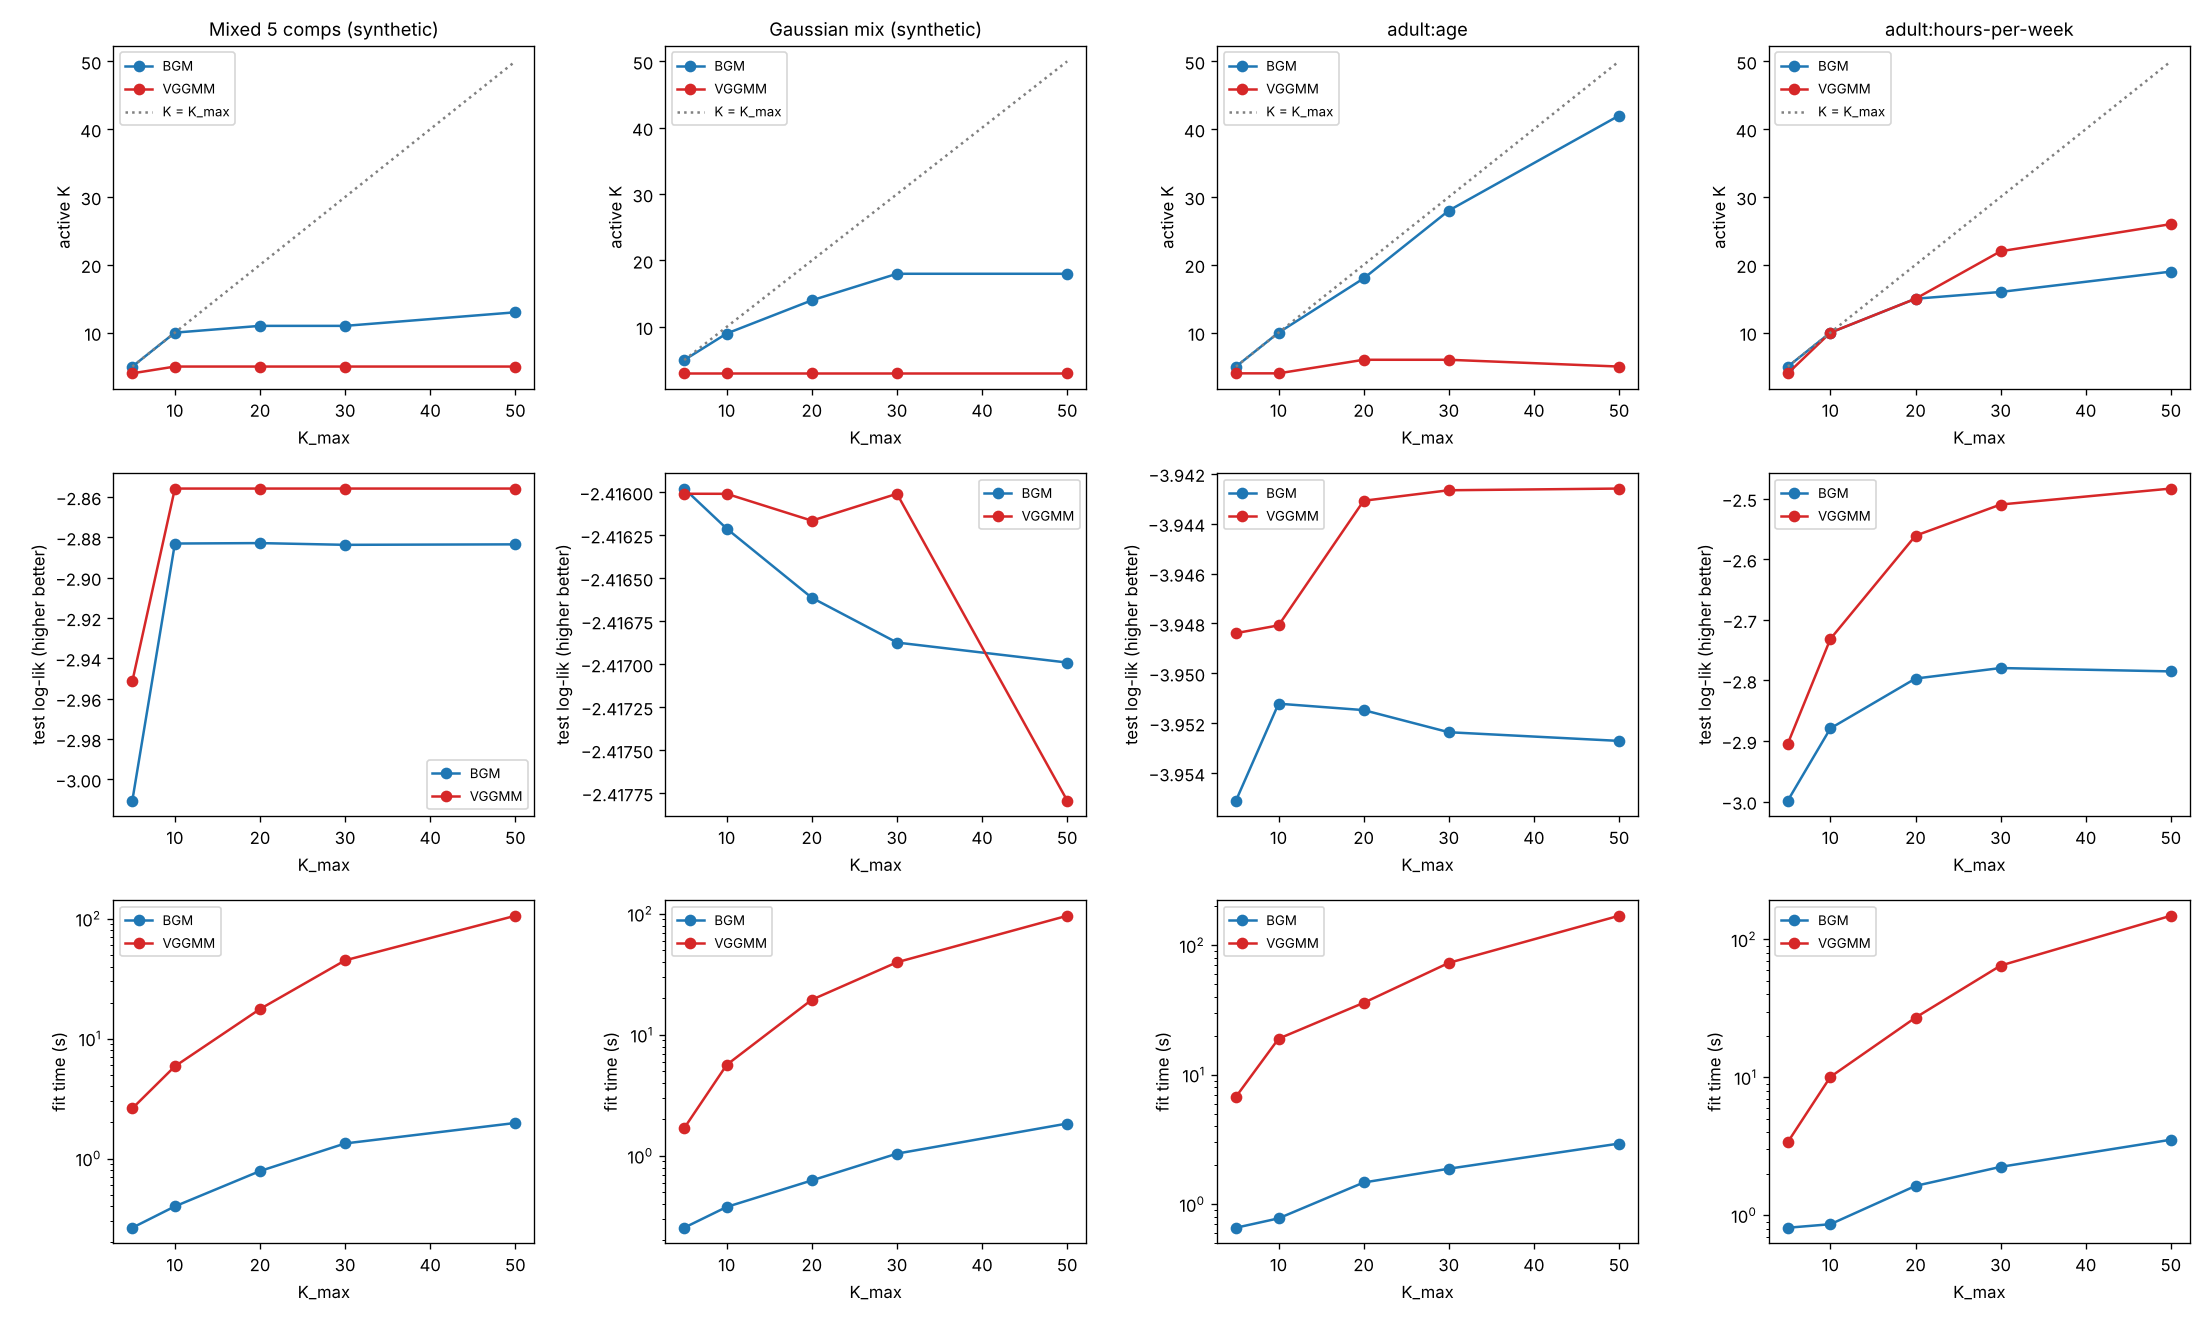
\includegraphics[width=\textwidth]{fig_kmax.png}
\caption{$K_{\max}\in\{5,10,20,30,50\}$에 따른 유효 성분 수(위), 평가 로그우도(가운데), 학습 시간(아래, 로그 눈금). 위 그림의 점선은 $K=K_{\max}$이다.}
\end{figure}

\begin{table}[h!]
\centering
\resizebox{\textwidth}{!}{\begin{tabular}{llrrrrr}
\toprule
데이터 & 항목 & $K_{\max}=5$ & $K_{\max}=10$ & $K_{\max}=20$ & $K_{\max}=30$ & $K_{\max}=50$ \\
\midrule
Mixed 5 comps (synthetic) & BGM 유효 $K$ & 5 & 10 & 11 & 11 & 13 \\
 & BGM ll & -3.011 & -2.883 & -2.883 & -2.884 & -2.883 \\
 & BGM 시간(s) & 0.3 & 0.4 & 0.8 & 1.3 & 2.0 \\
 & VGGMM 유효 $K$ & 4 & 5 & 5 & 5 & 5 \\
 & VGGMM ll & -2.951 & -2.856 & -2.856 & -2.856 & -2.856 \\
 & VGGMM 시간(s) & 2.6 & 5.9 & 17.7 & 45.0 & 106.1 \\
\addlinespace
Gaussian mix (synthetic) & BGM 유효 $K$ & 5 & 9 & 14 & 18 & 18 \\
 & BGM ll & -2.416 & -2.416 & -2.417 & -2.417 & -2.417 \\
 & BGM 시간(s) & 0.3 & 0.4 & 0.6 & 1.0 & 1.9 \\
 & VGGMM 유효 $K$ & 3 & 3 & 3 & 3 & 3 \\
 & VGGMM ll & -2.416 & -2.416 & -2.416 & -2.416 & -2.418 \\
 & VGGMM 시간(s) & 1.7 & 5.7 & 19.5 & 39.8 & 96.6 \\
\addlinespace
adult:age & BGM 유효 $K$ & 5 & 10 & 18 & 28 & 42 \\
 & BGM ll & -3.955 & -3.951 & -3.951 & -3.952 & -3.953 \\
 & BGM 시간(s) & 0.7 & 0.8 & 1.5 & 1.9 & 2.9 \\
 & VGGMM 유효 $K$ & 4 & 4 & 6 & 6 & 5 \\
 & VGGMM ll & -3.948 & -3.948 & -3.943 & -3.943 & -3.943 \\
 & VGGMM 시간(s) & 6.8 & 19.0 & 36.0 & 73.2 & 169.2 \\
\addlinespace
adult:hours-per-week & BGM 유효 $K$ & 5 & 10 & 15 & 16 & 19 \\
 & BGM ll & -2.998 & -2.879 & -2.797 & -2.780 & -2.785 \\
 & BGM 시간(s) & 0.8 & 0.9 & 1.6 & 2.2 & 3.5 \\
 & VGGMM 유효 $K$ & 4 & 10 & 15 & 22 & 26 \\
 & VGGMM ll & -2.904 & -2.731 & -2.561 & -2.510 & -2.483 \\
 & VGGMM 시간(s) & 3.4 & 10.1 & 27.1 & 64.6 & 148.5 \\
\addlinespace
\bottomrule
\end{tabular}}
\caption{$K_{\max}$ 비교의 수치. 학습 시간은 다른 작업 없이 단독으로 측정했다.}
\end{table}

\paragraph{관찰.}
\begin{itemize}
  \item \textbf{5성분 혼합과 정규 혼합(인공).}
    \begin{itemize}
      \item VGGMM은 $K_{\max}\ge10$이면 유효 성분이 각각 5와 3으로 일정하다(참값과 같다).
      \item BGM은 $10\to13$, $9\to18$로 늘지만 평가 로그우도는 그대로다. 정규 혼합에서는 두 방법의 차이가 $0.0002$ 이하다.
    \end{itemize}
  \item \textbf{adult age.}
    \begin{itemize}
      \item BGM은 유효 성분이 $K_{\max}$와 거의 같다($10\to42$). 로그우도는 오히려 조금 나빠진다($-3.951\to-3.953$).
      \item VGGMM은 4--6개이고, 로그우도는 $-3.948\to-3.943$이다.
    \end{itemize}
  \item \textbf{adult hours-per-week(반복되는 정수값이 많은 열).}
    \begin{itemize}
      \item 두 방법 모두 $K_{\max}$를 따라 성분이 늘어난다. VGGMM은 $10\to26$, BGM은 $10\to19$이다.
      \item 다만 VGGMM은 성분이 늘 때 로그우도가 크게 좋아진다($-2.732\to-2.483$, BGM은 $-2.879\to-2.785$).
      \item 40, 50, 60시간처럼 반복되는 값마다 폭 1짜리 상자가 생기므로, 데이터가 실제로 많은 성분을 필요로 하는 경우다. 성분 수가 \emph{적합도 향상 없이} 늘어나는 age의 BGM과는 성격이 다르다.
    \end{itemize}
  \item \textbf{학습 시간.}
    \begin{itemize}
      \item VGGMM은 $K_{\max}=10$에서 6--19초, $50$에서 97--169초였다.
      \item BGM은 각각 0.4--0.9초와 1.9--3.5초였다.
    \end{itemize}
\end{itemize}

\paragraph{$K_{\max}$를 무작정 키우면 안 되는 이유.}
\begin{enumerate}
  \item \textbf{BGM:} $K_{\max}$를 늘리면 유효 성분도 함께 늘지만 평가 로그우도는 거의 그대로이거나 조금 나빠진다. CTGAN에서는 연속 열 하나가 $1+K$차원(정규화 값 1개와 성분 원-핫 $K$개)이 되므로, 쓸모없는 성분은 생성기가 배워야 할 출력 차원만 늘린다.
  \item \textbf{VGGMM:} 유효 성분 수는 $K_{\max}\ge10$이면 거의 일정하다. 반면 계산량은 이동 탐색 때문에 $K_{\max}$에 대해 거의 제곱으로 늘어난다(5성분 데이터에서 $K_{\max}=10$일 때 5.9초, 50일 때 106초).
  \item \textbf{참고:} CTGAN 구현의 기본값은 10이다. 논문에 이 값의 근거가 있는지는 이번에 확인하지 못했다.
\end{enumerate}

\paragraph{제안.}
$K_{\max}=10$을 기본으로 쓰고, 유효 성분 수가 $K_{\max}$에 닿은 열에만 $K_{\max}$를 두 배로 늘려 다시 적합한다(``절단 점검'').
DP의 stick-breaking 절단은 쓰이지 않는 성분이 남아 있을 때 충분하다고 볼 수 있다(Ishwaran \& James, 2001). 실데이터 실험($K_{\max}=10$)에서 VGGMM이 상한 10에 닿은 경우는 반복되는 정수값이 많은 hours-per-week와 br2000 col10뿐이었다. 이런 열만 $K_{\max}=20$으로 다시 적합하면, 비용은 해당 열에만 든다.

\section{교수님 지적에 대한 응답}

\begin{enumerate}
  \item \textbf{``이웃을 묶는 것은 최적화가 아니다.''}
    \begin{itemize}
      \item 이동은 같은 목적함수(ELBO)가 \emph{같은 반복 횟수의 대조군}보다 커질 때만 받아들인다. 받아들인 뒤에도 같은 좌표 상승을 계속하므로 ELBO는 줄지 않는다.
      \item 하지만 \emph{어떤 후보를 시도할지}(이웃 쌍, 작은 성분)는 경험적 규칙이다. 이 부분의 지적은 타당하다.
    \end{itemize}
  \item \textbf{``$K_{\max}$가 커지면 시간이 폭증한다.''}
    \begin{itemize}
      \item 측정 결과도 그렇다. 5성분 데이터에서 $K_{\max}=10\to50$이면 시간이 약 18배 늘었다. BGM은 약 5배였다.
      \item 그래서 실용 범위는 $K_{\max}\approx10$이며, \S\ref{sec:kmax}의 절단 점검으로 보완하는 것을 제안한다.
    \end{itemize}
  \item \textbf{``BGM은 켤레이므로 $K_{\max}$를 키워도 적당한 $K$를 찾는다.''}
    \begin{itemize}
      \item 이번 실험에서는 그렇지 않았다. 참 분포가 BGM의 모형과 정확히 같은 정규 혼합(3성분)일 때도 BGM의 유효 성분은 $K_{\max}$를 따라 $5\to18$로 늘었다. adult age에서는 $5\to42$였다.
      \item 켤레성은 반복 한 번을 빠르게 해 주지만, 변분 최적화가 국소 최적에서 빠져나오게 해 주지는 않는다.
    \end{itemize}
\end{enumerate}

\section{결론과 다음 단계}
VGGMM은 첨도가 Gaussian과 다른 분포(두꺼운 꼬리, 평평한 봉우리, 0이나 정수값에 몰린 열)에서 BGM보다 참 분포에 훨씬 가깝게 맞춘다. 또 $K_{\max}$와 거의 무관하게 적은 수의 성분으로 같은 수준 이상의 적합도를 낸다.
반면 소표본에서 약하고, 계산 비용이 $K_{\max}$에 대해 크게 늘며, 이동 후보를 고르는 규칙이 경험적이라는 한계가 있다.
다음 단계로는 이동 없이 모든 갱신이 닫힌꼴인 ``켤레 구조'' 버전(형상 $\beta$를 격자 위의 범주형 사후로 두는 방식)을 같은 실험으로 비교할 계획이다. 이 버전은 아직 평가하지 않았다.

\paragraph{재현.} 모든 그림과 표는 \texttt{experiments/s14\_report.py}와 \texttt{s14\_tables.py}로 다시 만들 수 있다(시드 고정). 환경은 sklearn 1.9.1, scipy 1.18.1, numpy 2.5.4, rdt 2.1.0이다.

\begin{thebibliography}{9}\small
\bibitem{ij} H.~Ishwaran and L.~F. James. Gibbs sampling methods for stick-breaking priors. \emph{JASA}, 96(453):161--173, 2001.
\bibitem{ctgan} L.~Xu, M.~Skoularidou, A.~Cuesta-Infante, and K.~Veeramachaneni. Modeling tabular data using conditional GAN. \emph{NeurIPS}, 2019.
\bibitem{hughes} M.~C. Hughes and E.~B. Sudderth. Memoized online variational inference for Dirichlet process mixture models. \emph{NIPS}, 2013.
\end{thebibliography}
\end{document}
